\documentclass[12pt,a4paper]{article}
%\usepackage{ctex}
\usepackage{amsmath,amscd,amsbsy,amssymb,latexsym,url,bm,amsthm}
\usepackage{epsfig,graphicx,subfigure}
\usepackage{balance}
\usepackage{wrapfig}
\usepackage{mathrsfs, euscript}
\usepackage[usenames]{xcolor}
\usepackage{hyperref}
\usepackage[vlined,ruled,commentsnumbered,linesnumbered]{algorithm2e}
\usepackage{ulem}
\usepackage{url}
\usepackage{enumerate}

\newtheorem{theorem}{Theorem}[section]
\newtheorem{lemma}[theorem]{Lemma}
\newtheorem{proposition}[theorem]{Proposition}
\newtheorem{corollary}[theorem]{Corollary}
\newtheorem{exercise}{Exercise}[section]
\newtheorem*{solution}{Solution}
\theoremstyle{definition}


\numberwithin{equation}{section}
\numberwithin{figure}{section}

\renewcommand{\thefootnote}{\fnsymbol{footnote}}

\newcommand{\postscript}[2]
 {\setlength{\epsfxsize}{#2\hsize}
  \centerline{\epsfbox{#1}}}

\renewcommand{\baselinestretch}{1.0}

\setlength{\oddsidemargin}{-0.365in}
\setlength{\evensidemargin}{-0.365in}
\setlength{\topmargin}{-0.3in}
\setlength{\headheight}{0in}
\setlength{\headsep}{0in}
\setlength{\textheight}{10.1in}
\setlength{\textwidth}{7in}
\makeatletter \renewenvironment{proof}[1][Proof] {\par\pushQED{\qed}\normalfont\topsep6\p@\@plus6\p@\relax\trivlist\item[\hskip\labelsep\bfseries#1\@addpunct{.}]\ignorespaces}{\popQED\endtrivlist\@endpefalse} \makeatother
\makeatletter
\renewenvironment{solution}[1][Solution] {\par\pushQED{\qed}\normalfont\topsep6\p@\@plus6\p@\relax\trivlist\item[\hskip\labelsep\bfseries#1\@addpunct{.}]\ignorespaces}{\popQED\endtrivlist\@endpefalse} \makeatother



\begin{document}
\noindent

%========================================================================
\noindent\framebox[\linewidth]{\shortstack[c]{
\Large{\textbf{Computer Graphics Assignment 4}}}}
\begin{center}

\footnotesize{\color{blue}$*$ Name:Yongxi Huang  \quad Student ID:119033910011 \quad Email: huangyongxi@sjtu.edu.cn}
\end{center}

\noindent\textbf{Code will be uploaded to \\
	\url{https://github.com/Riften/SJTU-Computer-Graphics-2020-Assignments}\\
	 after deadline.}

\section{Question 1}
Describe the difference in appearance you would expect between a Phnog illumination model that used $(\bar{N}\cdot \bar{H})^n$ and one that used $(\bar{R}\cdot \bar{V})^n$.

\begin{solution}
	\begin{figure}[h]
		\centering
		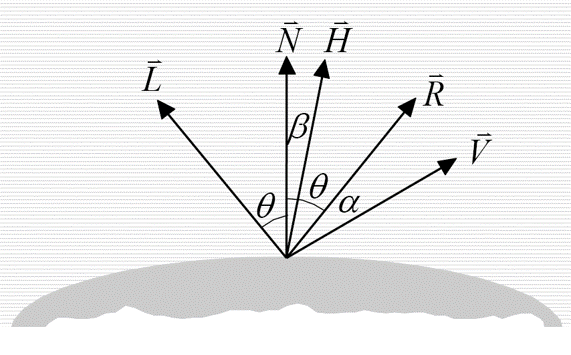
\includegraphics[width=0.5\textwidth]{PhongVectors.png}
		\caption{Vectors for calculating Phong shading}
		\label{fig1}
	\end{figure}
	The definitions of these vectors are as following
	\begin{align*}
	\bar{L}&: \text{Direction to the light source.}\\
	\bar{R}&:\text{Direction of reflection.}\\
	\bar{V}&:\text{Direction to the viewpoint.}\\
	\bar{N}&: \text{Surface normal.}\\
	\bar{H}&= \frac{\bar{L}+\bar{V}}{||\bar{L}+\bar{V}||}\\
	& \text{Halfway vector between the viewer and light-source vectors}
	\end{align*}
	The intuitive way to calculate specular hightlights is $(\bar{R}\cdot \bar{V})^n$. It gets the maximum when $\bar{R}=\bar{V}$, which is in line with common sence. However, $(\bar{N}\cdot \bar{H})^n$ also gets maximum when $\bar{R}=\bar{V}$. That means the brightest position of the specular hightlights is exactly the same when using these two formulas.
	
	But the size and intensity of hightlights would be different. Note that
	\begin{align*}
		\bar{R}\cdot \bar{V} &= \cos\alpha\\
		\bar{N}\cdot \bar{H} &= \cos\beta\\
		\beta &= \frac{\alpha + 2\theta}{2} - \theta = \frac{\alpha}{2}
	\end{align*}
	So there are $\bar{R}\cdot \bar{V} \leq \bar{N}\cdot \bar{H}$, and $\bar{R}\cdot \bar{V} = \bar{N}\cdot \bar{H}$ when $\bar{R} = \bar{V}$. In that case, with the same specular exponent $n$, Phong illumination model used $(\bar{N}\cdot \bar{H})^n$ would have a larger hightlight area than the one used $(\bar{R}\cdot \bar{V})^n$ as shown in Fig.\ref{fig2}.
	
	\begin{figure}[h]
		\centering
		\subfigure[$(\bar{N}\cdot \bar{H})^n$]{
			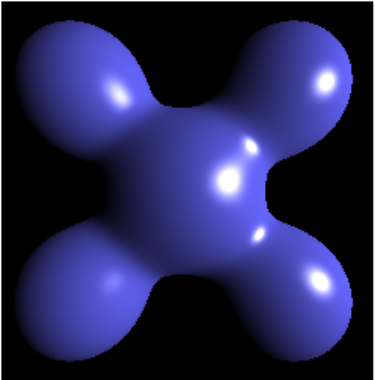
\includegraphics[width=0.3\linewidth]{BlinnPhong.png}
		}
		\subfigure[$(\bar{R}\cdot \bar{V})^n$]{
			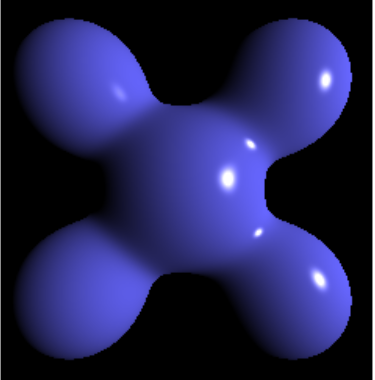
\includegraphics[width=0.3\linewidth]{Phong.png}
		}
	\caption{Phong illumination model used $(\bar{N}\cdot \bar{H})^n$ and $(\bar{R}\cdot \bar{V})^n$\cite{phongwiki}}
	\label{fig2}
	\end{figure}

	In fact, Phong shading using $(\bar{N}\cdot \bar{H})^n$ to calculate specular hightlights is called \textbf{Blinn-Phong Shading}\cite{phongwiki}.
	
	Another appearance difference between Blinn-Phong and Phong shading model occurs when $\alpha > \pi/2$. In that case, $\bar{R}\cdot \bar{V} < 0$ and the specular hightlight would be $0$ for Phong shading model. That would generate a sharp border of hightlights when specular exponent $n$ is small as shown in Fig.\ref{fig3}. In that case, Blinn-Phong is more similar with real sence.
	
	\begin{figure}[h]
		\centering
		\subfigure[Blinn Phong]{
			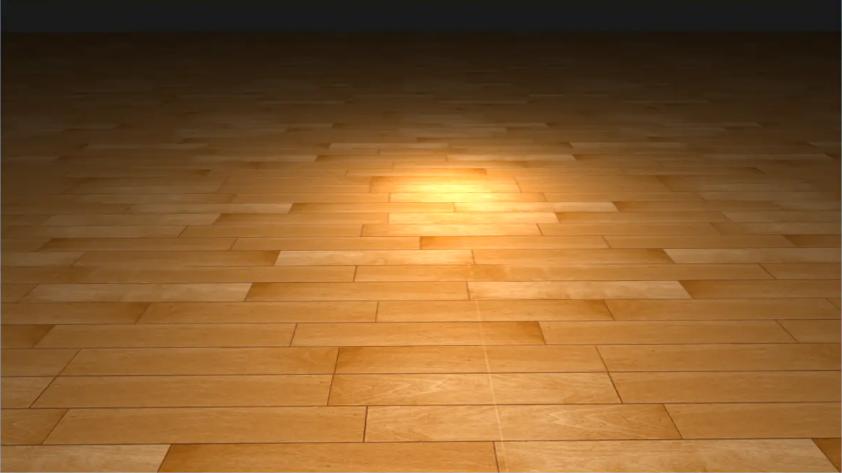
\includegraphics[width=0.4\linewidth]{BlinnPhong2.png}
		}
		\subfigure[Phong]{
			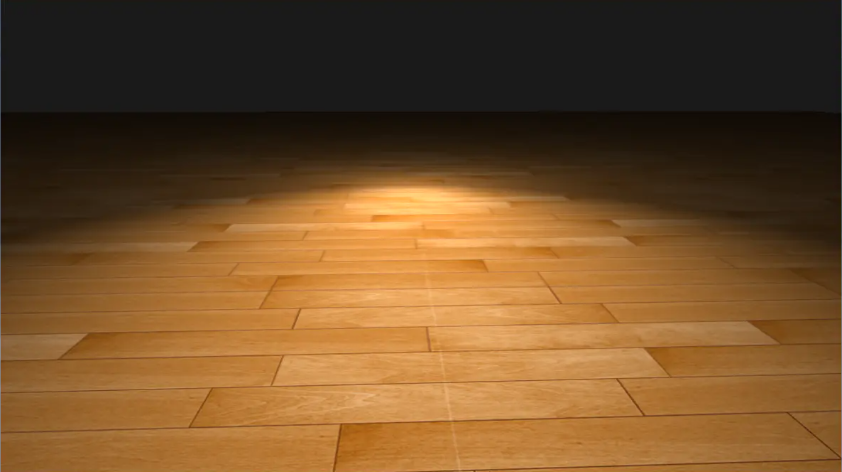
\includegraphics[width=0.4\linewidth]{Phong2.png}
		}
		\caption{Difference between Blinn Phong and Phong shading when $n=1$.\cite{blog}}
		\label{fig3}
	\end{figure}
	
\end{solution}

\section{Question 2}
\begin{enumerate}[a.]
	\item Prove that $\alpha=2\beta$ when all vectors of Fig.\ref{fig1} are coplanar.
	\begin{solution}
		That has been shown in \textbf{Question 1}.
		
		When $\bar{V}$ is lower than $\bar{R}$, there is
		\begin{align*}
			\beta &= \frac{\alpha + 2\theta}{2} - \theta = \frac{\alpha}{2}
		\end{align*}
		
		When $\bar{V}$ is between $\bar{L}$ and $\bar{R}$, there is
		\begin{align*}
			\beta &= \theta - \frac{2\theta-\alpha}{2}=\frac{\alpha}{2}
		\end{align*}
		
		When $\bar{V}$ is lower than $\bar{L}$, there is
		\begin{align*}
			\beta&=\theta + \frac{\alpha-2\theta}{2} = \frac{\alpha}{2}
		\end{align*}
		
		So that $\alpha=2\beta$ when all vectors are coplanar.
	\end{solution}
	\item Prove that this relationship is not true in general.
	\begin{solution}
		\begin{figure}[h]
			\centering
			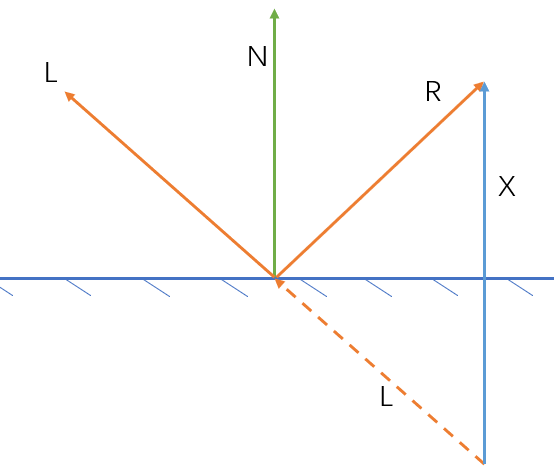
\includegraphics[width=0.5\linewidth]{reflect.png}
			\caption{Calculate reflected vector}
			\label{fig4}
		\end{figure}
		The basic idea is that $\bar{V}$ can be seen as the reflected vector of $\bar{L}$ about $\bar{H}$.
		
		First, there is a simple method to calculate reflected vector. As shown in Fig.\ref{fig4}, there is
		\begin{align*}
			\bar{X} &= 2(\bar{L}\cdot \bar{N})\bar{N}\\
			\bar{R} &= \bar{X} - \bar{L}\\
			&=2(\bar{L}\cdot \bar{N})\bar{N}- \bar{L}
		\end{align*}
		
		If we see $\bar{V}$ as the reflected vector of $\bar{L}$ about $\bar{H}$, there is
		\begin{align*}
			\bar{V} = 2(\bar{L}\cdot \bar{H})\bar{H}- \bar{L}
		\end{align*}
		
		So that
		\begin{align}
			\bar{R}\cdot\bar{V} &= 2(\bar{L}\cdot \bar{H})(\bar{H}\cdot \bar{R})- \bar{L}\cdot \bar{R}\\
			&=4(\bar{L}\cdot \bar{N})(\bar{L}\cdot \bar{H})(\bar{N}\cdot \bar{H}) - 2 (\bar{L}\cdot \bar{N})^2 - 2(\bar{L}\cdot \bar{H})^2 + \bar{L}^2
			\label{eq1}
		\end{align}
		
		Define
		\begin{align*}
			a &= -2\\
			b &= 4(\bar{L}\cdot \bar{N})(\bar{N}\cdot \bar{H})\\
			c &= \bar{L}^2- 2 (\bar{L}\cdot \bar{N})^2\\
			x &= \bar{L}\cdot \bar{H}
		\end{align*}
		Then equation \ref{eq1} would be 
		\begin{align}
			\bar{R}\cdot\bar{V} =\cos\alpha= ax^2+bx+c
			\label{eq2}
		\end{align}
		
		Assume that $\bar{H}'$ is a halfway vector that is not coplanar with $\{L,N,H\}$. It can be seen from a coplanar vector $\bar{H}$ rotating around $\bar{N}$.	Note that when $\bar{H}$ rotating around $\bar{N}$, $(\bar{N}\cdot \bar{H})$ will remain unchanged.
		
		In that case, when $\bar{H}$ is rotating around $\bar{N}$, both $\{a,b,c\}$ would be unchanged constant. Only $x$ is changing unless $\bar{L}=\bar{N}$.
		
		So when $\bar{H}$ is rotating around $\bar{N}$, $\beta$ will remain unchanged, while $\alpha$ is changed according to equation \ref{eq2}. So $\alpha \neq 2\beta$ when $\bar{V}$ is not conplanar with $\{L,N,H\}$.
		
	\end{solution}
\end{enumerate}

\bibliography{ref}{}
\bibliographystyle{IEEEtran}
%========================================================================
\end{document}
